\documentclass[11pt,a4paper]{article}
\oddsidemargin 0.1 cm \evensidemargin 0.1cm \textwidth 16cm
\textheight24cm
\setlength{\topmargin}{0pt}\setlength{\headsep}{0pt}\pagestyle{empty}

\usepackage{graphicx}
\usepackage{variations}
\usepackage{enumerate}
\usepackage{amssymb}
\usepackage[latin1]{inputenc}  
\usepackage{fontenc}   
\usepackage{amsmath}
\usepackage{amsthm}
\usepackage{amsthm}
\usepackage{xypic}
\usepackage{variations}
%\usepackage{fancyhdr}
%\usepackage{xcolor}
%\usepackage{pstricks-add}
\usepackage[francais]{babel}
%\usepackage[french]{babel}
\newtheorem{defi}{D\'{e}finition}
\newtheorem{thm}{Th\'{e}or\`{e}me}
\newtheorem{rmq}{Remarque}
\newtheorem{prop}{Propri\'{e}t\'{e}}
\newtheorem{prop-def}{Propri\'{e}t\'{e}-D\'{e}finition}
\newtheorem{ex}{Exemple}
\newtheorem{exs}{Exemples}
\newtheorem{exer}{Exercice}
%\newtheorem{proof}{D\'{e}monstration}
\def\di{\displaystyle}
\newcommand{\vtab}{\rule[-0.4em]{0pt}{1.2em}}
\usepackage[top=0.5cm,bottom=0.5cm,right=1.5cm,left=1.5cm]{geometry}
\usepackage{pstricks,pst-plot} 
%\usepackage{framed}
\usepackage{amsmath}
%\usepackage{amssymb}
\usepackage{fancyhdr}
\usepackage{fancybox}
\usepackage{multicol}
%\usepackage{xcolor}
\usepackage{epsfig}
\usepackage{pifont}
%\usepackage[framed]{ntheorem}
%\usepackage[frenchb]{babel}
\usepackage{tabularx}
\def\R{{\mathbb R}}
\newtheorem{Rem}{Remarque}
\newcommand{\V}{\overrightarrow}
\newcommand{\Rep}{(O;\V{\imath};\V{\jmath})}
\newcommand{\Coor}[2]{\begin{pmatrix} #1\\#2 \end{pmatrix}}

\begin{document}
\title{}         % Enter your title between curly braces
\author{}        % Enter your name between curly braces
\date{}          % Enter your date or \today between curly braces
\maketitle

\indent\vspace{-3cm}
$$\fbox{\text{\begin{Large}Vecteurs - Feuille d'exercices niveau 3 \end{Large}}}$$
     
\hfill\\[0.2cm]


\noindent\underline{\textbf{Exercice 1 :}}\\[0.1cm]
Soient $A$ et $B$ deux points du plan. Soit $O$ le milieu de $[AB]$. 
\begin{enumerate}
\item Noah a r�ussi � tracer deux points $E$ et $F$ v�rifiant les deux conditions suivantes :
$$\text{$\V{AE}+\V{AF}=\V{AB}$ \ \ et \ \ $(EF)\perp (AB)$.}$$
	\begin{enumerate}[$a.$]
	\item Quelle conclusion sur la nature de $AEFB$ peut-on en d�duire de la relation $\V{AE}+\V{AF}=\V{AB}$ ?
	\item Quelle est la nature exacte du quadrilat�re $AEBF$ ?
	\end{enumerate}
\item Construire un tel quadrilat�re $AEBF$. 
\end{enumerate}
\hfill\\[-0.5cm]

\noindent\underline{\textbf{Exercice 2 :}}\\[-1.1cm]

\begin{minipage}{0.7\linewidth}
\noindent Sur la figure ci-contre, les droites $(EF)$ et $(BC)$ sont parall�les, ainsi que les droites $(EH)$ et $(AC)$.
\begin{enumerate}
\item Quelle est la nature du quadrilat�re $CFEH$ ?
\item D�montrer que $\V{BH}+\V{EF}=\V{BC}$ et que $\V{EH}+\V{AF}=\V{AC}$.
\end{enumerate}
\end{minipage}\hfill
\begin{minipage}{0.3\linewidth}
$$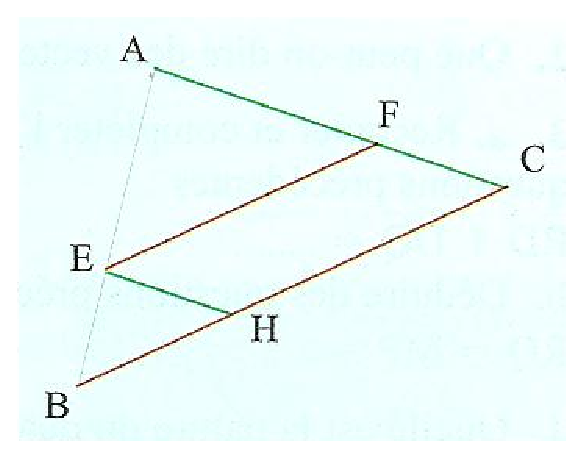
\includegraphics[scale=0.5]{exo2.eps}$$
\end{minipage}
\hfill\\[-0.8cm]

\noindent\underline{\textbf{Exercice 3 :}}\\[0.1cm]
Soit $ABCD$ un carr� de centre $O$.
\begin{enumerate}
\item Construire le point $M$ tel que $\V{OM}=\V{OA}+\V{OB}$. Quelle est la nature du quadrilat�re $OAMB$ ?
\item Construire les points $N$, $P$ et $Q$ d�finis par 
$$\text{$\V{ON}=\V{OB}+\V{OC}$ \ \ , \ \ $\V{OP}=\V{OC}+\V{OD}$ \ \ et \ \ $\V{OQ}=\V{OD}+\V{OA}$.}$$
\item Quelle est la nature exacte du quadrilat�re $MNPQ$ ?
\end{enumerate}
\hfill\\[-0.3cm]

\noindent\underline{\textbf{Exercice 4 :}}\\[0.1cm]
Soient $A$, $B$ et $C$ trois points donn�s. D�terminer le point $M$ tel que $\V{AC}=\V{AM}+\V{BC}$.
\hfill\\  

\noindent\underline{\textbf{Exercice 5 :}}\\[0.1cm] 
Soient $A$, $B$ et $C$ trois points donn�s. On consid�re le point $M$ tel que $\V{CM}=\V{BA}+\V{CA}$.
\begin{enumerate}
\item D�montrer que $\V{AM}=\V{BA}$. 
\item Que peut-on en d�duire pour le point $M$ ?
\end{enumerate}
\hfill\\[-0.3cm]

\noindent\underline{\textbf{Exercice 6 :}}\\[0.1cm]
Soit $ABC$ un triangle �quilat�ral, $D$ un point quelconque du plan, $I$ le milieu de $[DB]$ et $J$ le milieu de $[DC]$.
\begin{enumerate}
\item Construire le sym�trique $E$ de $A$ par rapport � $I$ et $F$ le sym�trique de $A$ par rapport � $J$.
\item  D�montrer que $\V{AD}=\V{BE}$ et que $\V{CF}=\V{AD}$.
\item Quelle transformation am�ne $ABC$ sur $DEF$ ? Quelle est la nature du triangle $DEF$ ?
\end{enumerate}
\hfill\\

\noindent\underline{\textbf{Exercice 7 :}}\\[0.1cm]
Soient $A$, $B$, $C$ et $D$ quatre points du plan v�rifiant :
$$\V{BA}+\V{CB}+\V{DC}=\V{CA}+\V{DB}-\V{CD}.$$
D�montrer que les points $B$ et $D$ sont confondus.
\hfill\\

\newpage

\noindent\underline{\textbf{Exercice 8 :}}\\[0.1cm] 
Soient $A$, $B$, $C$ et $D$ quatre points du plan. Soient $I$, $J$, $K$ et $L$ les milieux respectifs des segments $[AC]$, $[BD]$, $[AD]$ et $[BC]$.
\begin{enumerate}
\item Montrer que $\V{AB}+\V{CD}=\V{AD}+\V{CB}=2\V{IJ}$.\\
(Remarque : $2\V{IJ}=\V{IJ}+\V{IJ}$)
\item Montrer que $\V{AB}-\V{CD}=\V{AC}-\V{BD}=2\V{KL}$.\\
(Remarque : $2\V{KL}=\V{KL}+\V{KL}$)
\end{enumerate}
\hfill\\[-0.5cm] 

\noindent\underline{\textbf{Exercice 9 : }}\\[0.1cm]
Soit $ABCD$ un parall�logramme. Soit $E$ le milieu de $[BC]$ et $F$ le milieu de $[DC]$.
\begin{enumerate}
\item Montrer que $\V{AC}+\V{BD}=2\V{BC}$.
\item Montrer que $\V{AE}+\V{AF}=\di\frac{3}{2}\V{AC}$.
\end{enumerate} 
\hfill\\[-0.5cm]

\noindent\underline{\textbf{Exercice 10 : }}\\[0.1cm]
Soit $ABC$ un triangle. 
\begin{enumerate}
\item Construire les points $E$ et $F$ v�rifiant :
$$\text{$\V{AE}=-\V{AC}$ \ \ et \ \ $\V{AF}+\V{BF}-\V{CF}=\V{0}$.}$$ 
\item D�montrer que $AFBC$ et $AEFB$ sont des parall�logrammes.
\end{enumerate}
\hfill\\[-0.5cm]


\noindent\underline{\textbf{Exercice 11 : }}\\[0.1cm]
Soit $ABC$ un triangle. Construire les points $E$ et $F$ v�rifiant :
$$\V{AE}=\V{BE}+\V{CE} \ \ \ \text{et} \ \ \ \V{AF}+2\V{BF}=\V{CF}$$



\noindent\underline{\textbf{Exercice 12 : }}\\[0.1cm]
Soit $ABC$ un triangle. 
\begin{enumerate}
\item Placer le point $D$ tel que $\V{AD}=\V{AB}+2\V{AC}$.
\item Placer le point $E$ tel que $\V{AE}+2\V{BE}-\V{CE}=\V{0}$.
\item Placer le point $F$ tel que $\V{BF}=\V{AF}+\V{CF}$.
\item Que peut-on dire du quadrilat�re $AFCB$ ? Le d�montrer.
\end{enumerate}
\hfill\\[-0.5cm]


\noindent\underline{\textbf{Exercice 13 : }}\\[0.1cm]
Soit $ABCD$ un quadrilat�re quelconque. Soit $I$ le milieu de $[AB]$ et $J$ le milieu de $[CD]$. Soit $E$ le point v�rifiant :
$$\V{EA}+\V{EB}+\V{EC}+\V{ED}=\V{0}.$$ 
Montrer que $E$ est le milieu de $[IJ]$.
\hfill\\[0.2cm]

\noindent\underline{\textbf{Exercice 14 : }}\\[0.1cm]
Soit $ABC$ un triangle. Soit $I$ le milieu de $[AB]$ et $J$ le milieu de $[IC]$.\\
Montrer que $\V{JA}+\V{JB}+\V{JC}=\V{JI}$.

\end{document}
